\section{Methods description}
In this section, we outline a strategy for estimating the time evolution of the ratio $r=M_{\rm PNS}/R_{\rm PNS}^2$ of the mass of the proto-neutron star (PNS) and its squared radius (in units of solar mass and km) from the gravitational wave observations.
An integral part of this strategy is the universal relationship between the characteristic frequency of the PNS oscillation $f$, $g$ and $p$ modes and a combination of the mass, the radius of the PNS, the shock radius and the total mass inside the shock as demonstrated by \cite{Torres:2019}. In this paper we focus on the $^2g_2$ mode. 

Using 25 1D simulations obtained with the {\sc AENUS-ALCAR }code \cite{} and the {\sc CoCoNuT} \cite{} code, we parametrize the ratio with a cubic polynomial regression with heteroscedastic errors
%Here we are using the data from \textcolor{red}{only {\sc AENUS-ALCAR} or both?, maybe colour-code the two groups of data points } to fit a cubic polyn
\begin{equation}
r_i=\beta_1 f_i + \beta_2 f_i^2 +\beta_3 f_i^3 + \epsilon_i
\end{equation}
where $\epsilon_i$ are assumed to be independent zero-mean Gaussian errors with  variances $\sigma_i^2$ that increase with frequency $f_i$. The model for frequency-dependent variances is
\begin{equation}
\log \sigma_i=\alpha_0+ \alpha_1 f_i + \alpha_2 f_i^2 + \delta_i
\end{equation}
with independent and identically zero-mean Gaussian errors $\delta_i$. The R-package LMVAR
\cite{lmvar:2019} that implements a maximum likelihood approach was used to fit the model. The best
fitting model amongst polynomials of degree 1, 2, and 3  was chosen according to the Aikaike information
criterion with coefficients given in Table \ref{tab:model},

\begin{equation}\label{eq:universal}
r_i = \beta_1 f_i + \beta_3 f_i^3 + \epsilon_i
\end{equation}

The best-fitting model achieves a coefficient of determination of $R^2=0.9812$.
The data and fit of the model including 95\% confidence bands are displayed in Figure \ref{Fig:LMVAR}.

\begin{table}[h]
  \begin{tabular}{lll}
    \hline
    Coefficient & Estimate & standard error \\
    \hline
    $\beta_1$   & $6.09 \times 10^{-7}$ & $1.75 \times 10^{-8}$ \\
    $\beta_3$   & $6.24 \times 10^{-13}$ & $8.79 \times 10^{-15}$ \\
    \hline
  \end{tabular}
\label{tab:model}
\caption{Estimate and standard error of the coefficients of the best fit model describing the ratio $r=M_{\rm PNS}/R_{\rm PNS}^2$ as function of the frequency of the $^2g_2$ mode.}
\end{table}

\begin{figure}
 \centering
 \includegraphics[width=0.5\textwidth,height=0.3\textheight]{model.pdf}
 \caption{Data from 25 1D simulations {\sc AENUS-ALCAR } and {\sc CoCoNuT}  code, solid line is the maximum likelihood estimate of heteroscedastic cubic model with 95\% confidence bands.} \label{Fig:LMVAR}
\end{figure}

We consider the gravitational wave signal {\tt s20-gw-10kpc} described in Section \ref{sec:simulation}, originally sampled at 20 kHz but resampled to the LIGO sampling rate of 16384 Hz.
A spectrogram of this signal is shown in Figure \ref{fig:spectrogram} based on autoregressive estimates of the local spectra for successive time intervals of 
\textcolor{red}{length 200} with a \textcolor{red}{ 90\%} overlap.The dominant emission mode correspondes to the $\mbox{ }^2 g_1$-mode \cite{} and we have developed a time-frequency method to track the ridge $m(t)$ in the spectrogram, taking into account that it is monotonically increasing. Starting from either the left- or right-most column of the time-frequency  matrix we identify and trace the sequence of amplitude peaks within a certain frequency band given the monotonicity constraint. \textcolor{red}{Are more details regarding the ridge tracking required here?}

\begin{figure}
 \centering
 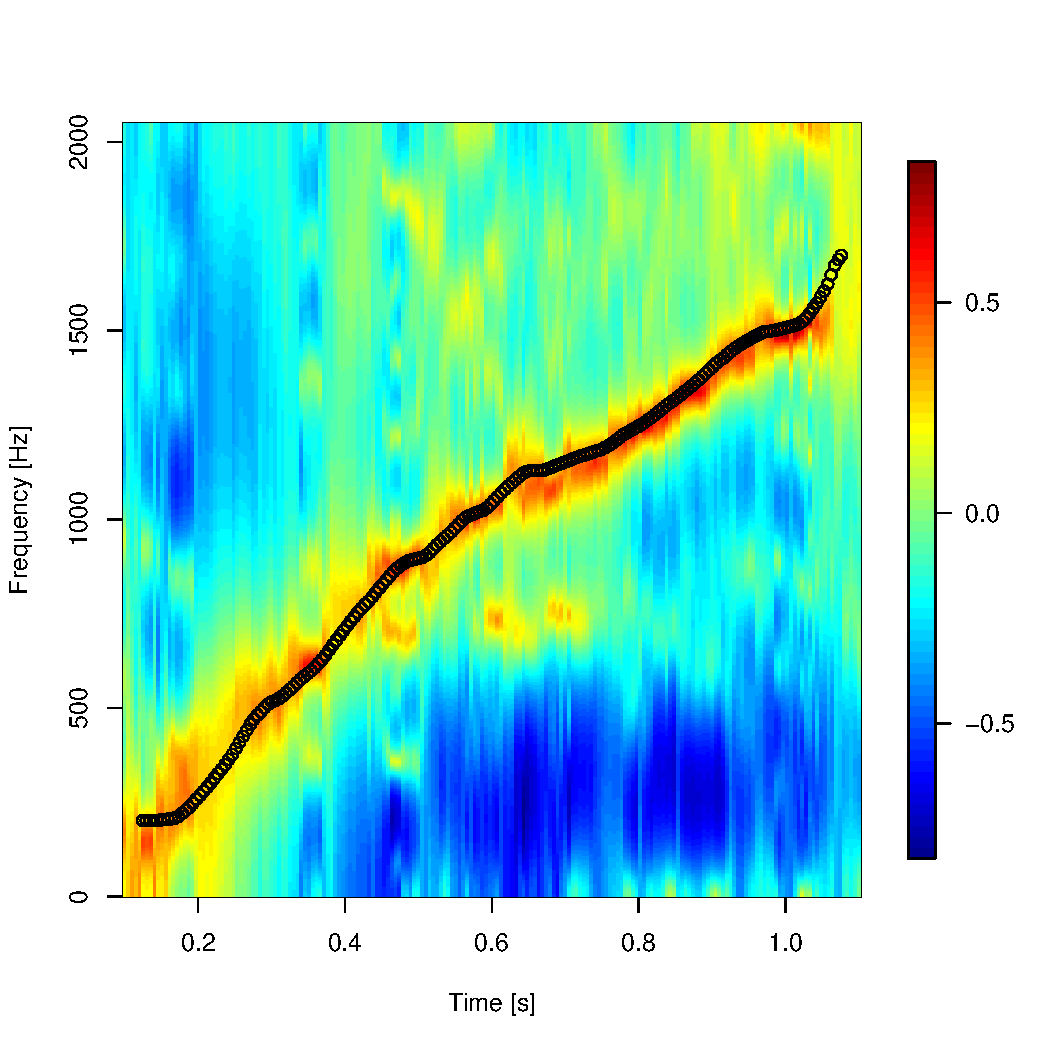
\includegraphics[width=0.5\textwidth,height=0.3\textheight]{plots/spectrogram.pdf}
 \caption{Spectrogram} \label{fig:spec}
\end{figure}



We identify the instantaneous frequency $f(t_i)$ corresponding the  ridge $m(t_i)$ for the midpoint $t_i$ of each local time interval of the spectrogram and interpolating $f(t)$
for values in between the $t_i$. Now we can use the universal relationship in (\ref{eq:universal}) to obtain estimates of the time evolution of the
ratios together with 95\% confidence intervals. These are given in Figure \ref{fig:xx} \textcolor{red}{insert figure} where the black points are the true ratio values, the red points the
estimates and the grey bands represent 95\% confidence bands. In this case without any noise, the coverage of our 95\% confidence band is xx\%.

In the following simulation study we explore how accurately we can estimate the parameters when the gravitational wave signal is embedded in noise.
For that purpose, we inject the gravitational wave signal into  simulated Advanced LIGO noise using the noise power spectral density \textcolor{red}{insert formula} for varying
SNRs, respectively distances to the source. We estimate the coverage probability of the 95\% confidence band by calculating the proportion of times that the true ratio lies outside one of the pointwise 95\% confidence intervals.
These coverage probabilities together for varying SNRs are given in Table \textcolor{red}{insert Table} and displayed in the form of boxplots in Figure \textcolor{red}{insert Figure}


\subsection{G-mode reconstruction}

Given the spectrogram and an specified time interval for the g-mode reconstruction, our proposal method works as follows.  The starting point must be specified.  It can be either at the beginning or at the end of the signal.  Then, in one of these extremes, the maximum energy value is identified, registering its frequency.  This is done independently for a number of consecutive time intervals.  Then we calculate the median of these frequency values, providing a robust starting value for the g-mode reconstruction.

The starting frequency value is the first g-mode estimate for the first or the last time interval, depending on the specified starting location.  If the reconstruction is set to start at the beginning of the signal, the reconstruction will be done progressively over the time intervals, where each maximum frequency value will be calculated within a frequency range specified by the previous g-mode estimate.  Given the non-decreasing behaviour of the true g-mode values, the g-mode estimates will be forced to be greater or equal than the one estimated for its previous time interval, and lower than a specified upper limit.  As a result, the g-modes estimates will be a non-decreasing sequence of frequency values. 

If the reconstruction is set to start at the end of the signal, the g-modes will be estimated backward in time.  Each maximum frequency is calculated within a range determined by its successor (in time) g-mode estimate.  These estimates are forced to be lower or equal than its successor (in time) estimate, but greater than a specified lower limit. Thus, a non-decreasing sequence of g-mode estimates is guaranteed.

This g-mode reconstruction method works if and only if the signal is strong enough to provide information about the g-mode, which is reflected in the spectrogram.

\subsection{ Confidence bands}
Given the sequence of g-mode estimates, the confidence band will be calculated by using the model defined in \eqref{eq:universal}. The g-mode estimates are frequency values which we use as predictors in the model in order to generate confidence intervals for the ratios. Since the g-mode estimates are indexed by time, the confidence intervals for the ratios are too.  Thus, we generate the confidence band by interpolating the lower and upper limits of the collection of consecutive confidence intervals, which will be valid for the time range of the g-mode estimates.  This confidence band is used to estimate the coverage probabilities in our simulation studies presented below.  




